% !TEX encoding = UTF-8
% !TEX TS-program = pdflatex
% !TEX root = ../../tesi.tex

\section{Lo standard ERC721 per Hotmoka}
Dato che Hotmoka è una \textit{blockchain} ancora giovane è risultato necessario lo sviluppo dello standard ERC721 per Hotmoka, dato che non ne ha uno. Non ho implementato tutto lo standard, ma solamente determinate componenti che risultavano necessarie per l'implementazione successiva del contratto per la gestione degli NFT.

\subsection{Progettazione}
Per quanto riguarda la progettazione dello standard ERC721 per Hotmoka, ho preso ispirazione dall'implementazione realizzata dall'azienda OpenZeppelin che lo ha sviluppato per Ethereum. L'unico \textit{design pattern} utilizzato è il \textbf{\textit{Guard Check}}. \\

Per aiutarmi e realizzare un'architettura complicata come quella dello standard ERC721, ho preso spunto anche dall'implementazione, già realizzata, dello standard ERC20 (standard per la gestione di \textit{token} fungibili) in Takamaka.

% \clearpage
\begin{figure}[h!]
  \centering
  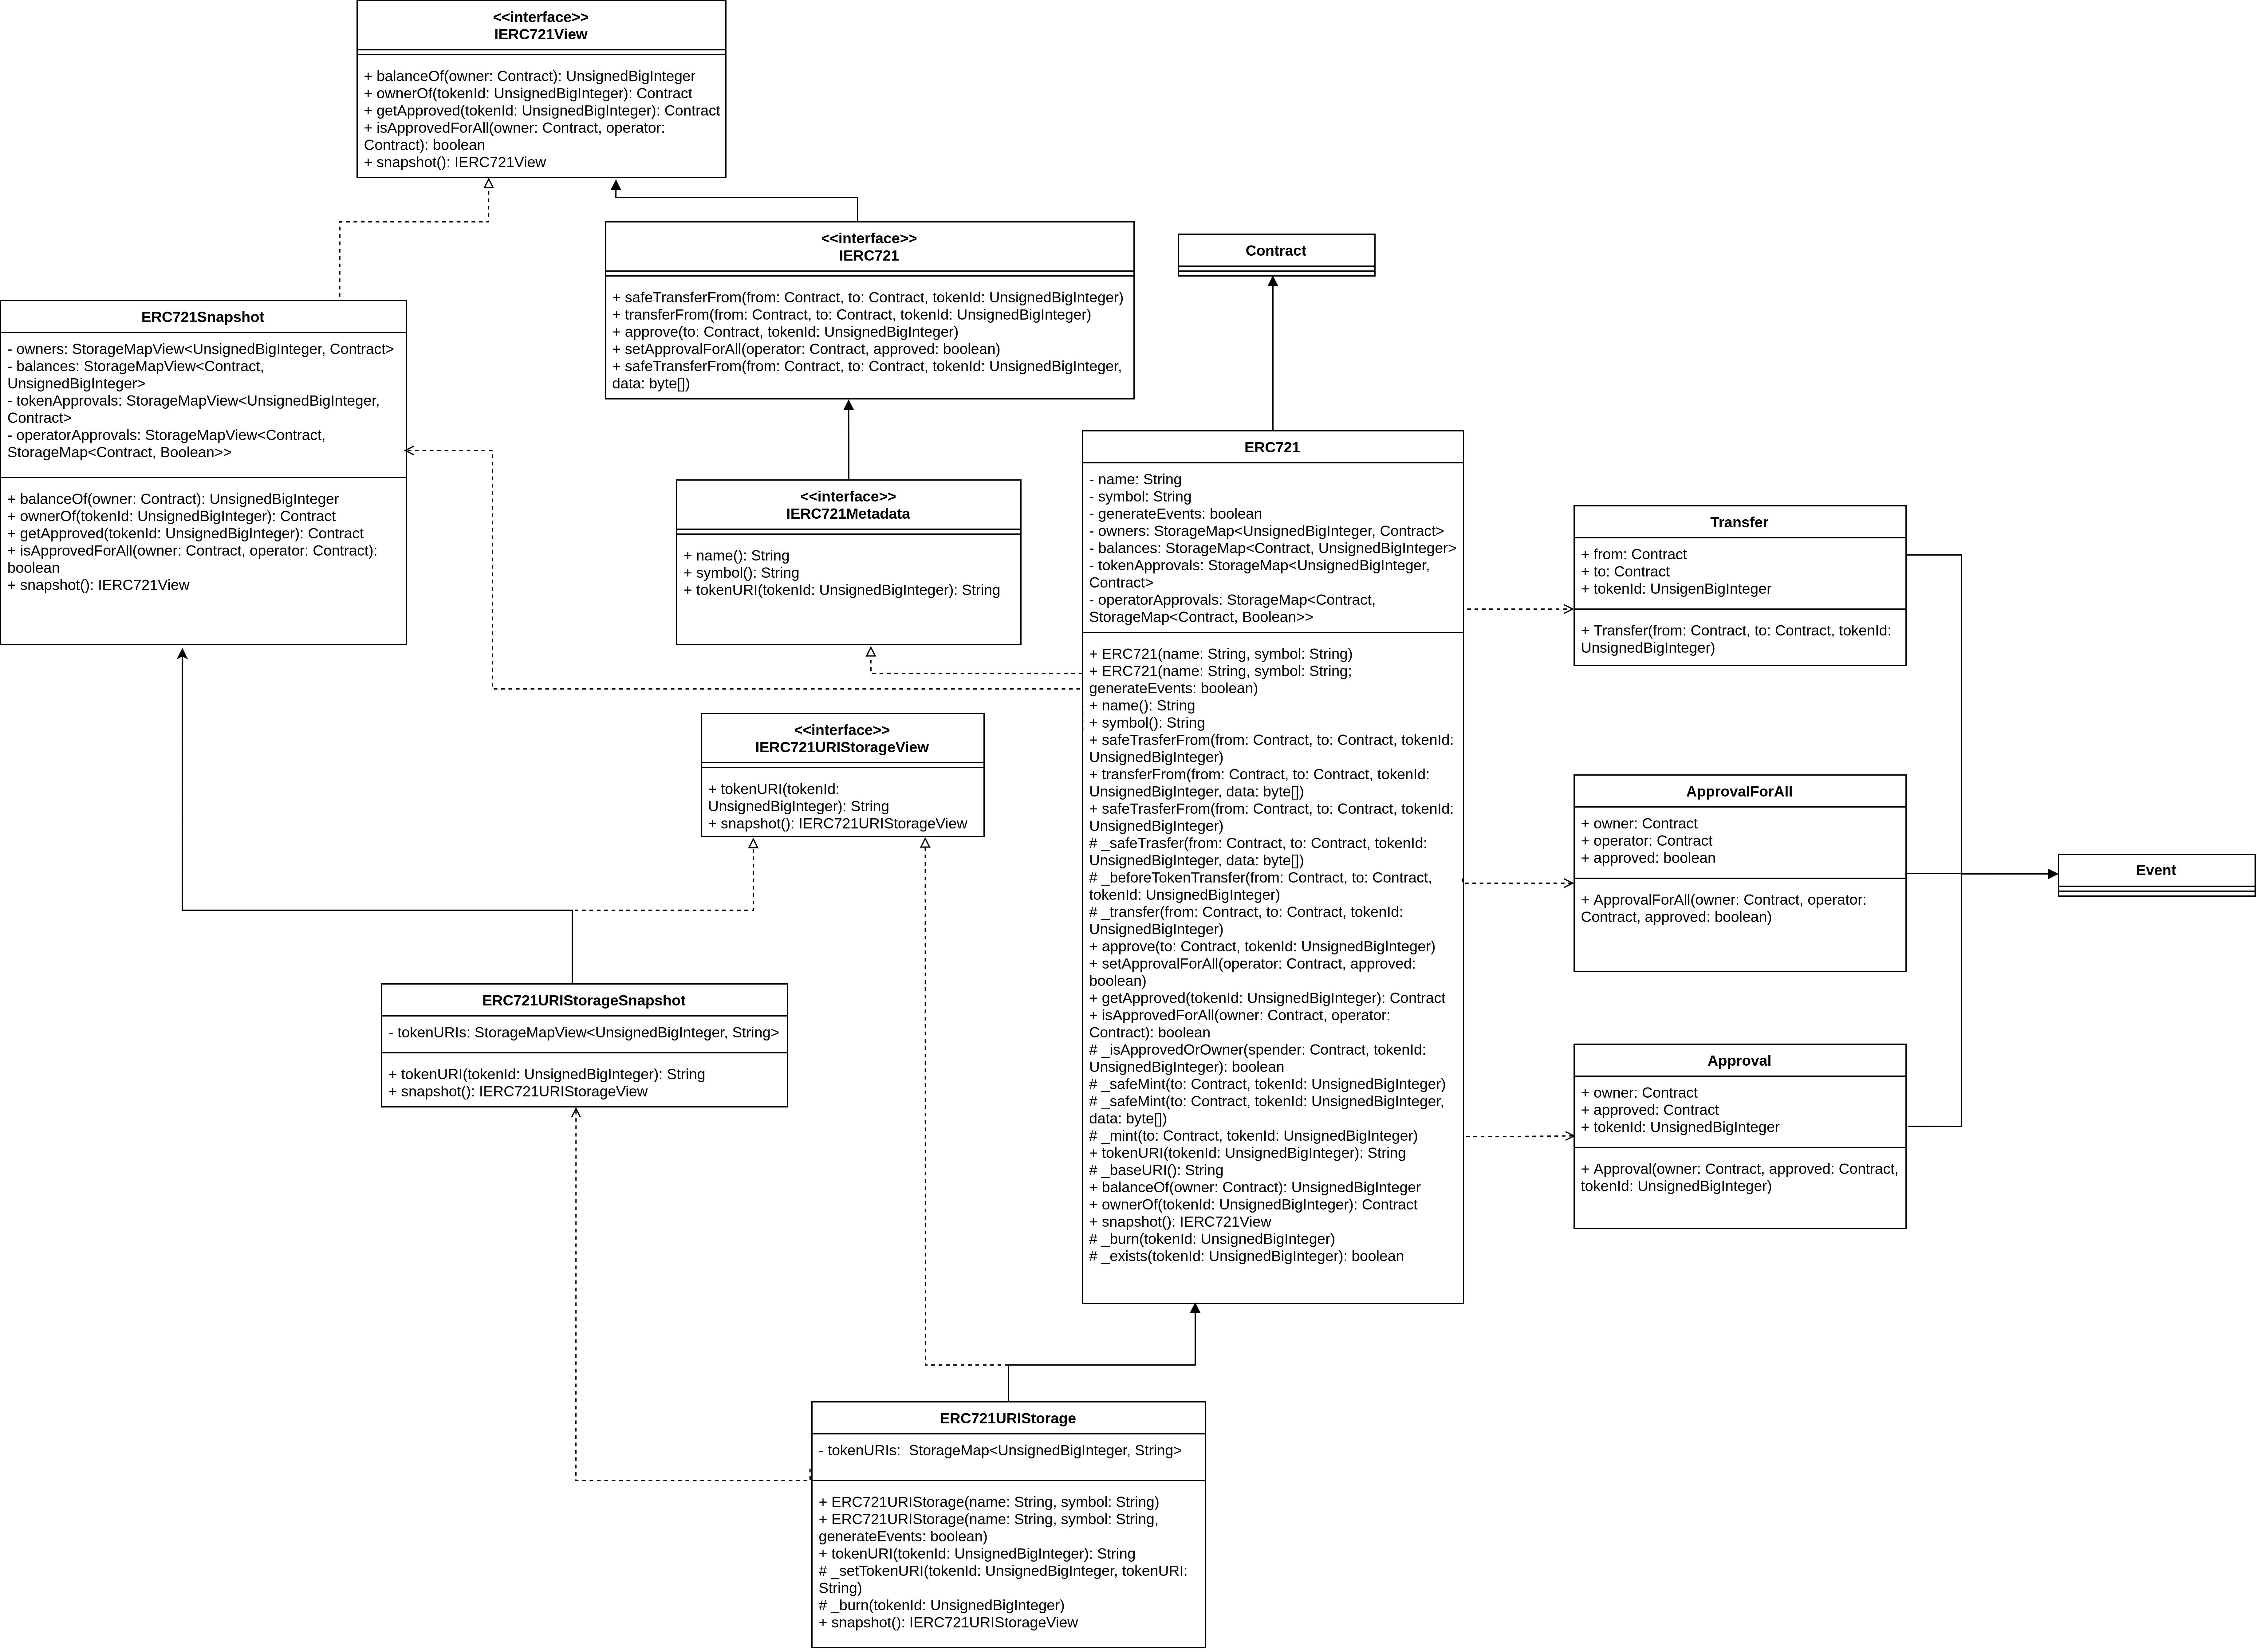
\includegraphics[width=\textwidth]{capitolo3/class-diagram/erc721-hotmoka-class-diagram.png}
  \caption{Diagramma delle classi dell'implementazione dello standard ERC721 per Hotmoka}
  \label{fig:erc721-hotmoka-class-diagram}
\end{figure}

Come si può vedere dal diagramma delle classi (figura \ref{fig:erc721-hotmoka-class-diagram}) per permettere l'esecuzione dello \textit{Snapshot} dello stato attuale della \textit{blockchain}, sono state dichiarate delle interfacce separate che racchiudono solo le funzioni che sono targate \textit{view}. In questo modo chiunque potrà eseguire quelle funzioni in una copia dello stato attuale della rete, senza avere inconsistenze.

\subsection{Codifica}
In seguito alla fase di progettazione, sono passato alla fase di codifica.
Inizialmente ho definito tutte le interfacce individuate in fase di progettazione e, in seguito, sono passato alla definizione delle classi dove ho prima definito tutte le firme dei metodi per poi eseguire l'implementazione. \\

% \begin{figure}[h!]
%   \centering
%   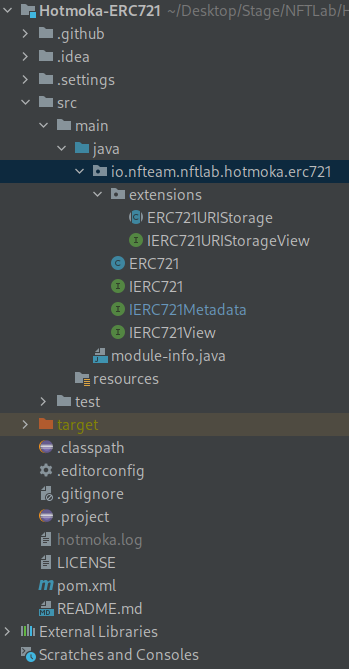
\includegraphics[width=0.3\textwidth]{capitolo3/erc721-hotmoka/erc721-hotmoka-structure.png}
%   \caption{Struttura del progetto dello standard ERC721 per Hotmoka}
% \end{figure}

Meritevole di attenzione è l'implementazione del sistema dello \textit{Snapshot}. Come si può vedere in figura \ref{fig:erc721-snapshot} viene eseguito lo \textit{snapshot} dello stato attuale e vengono implementati i metodi per leggerlo. Questo è un grande vantaggio che ha Takamaka rispetto a Solidity, infatti in questo caso lo \textit{snapshot} può essere eseguito in tempo O(1), mente in Solidity è quasi impossibile realizzarlo così facilmente.

\begin{figure}[h!]
  \centering
  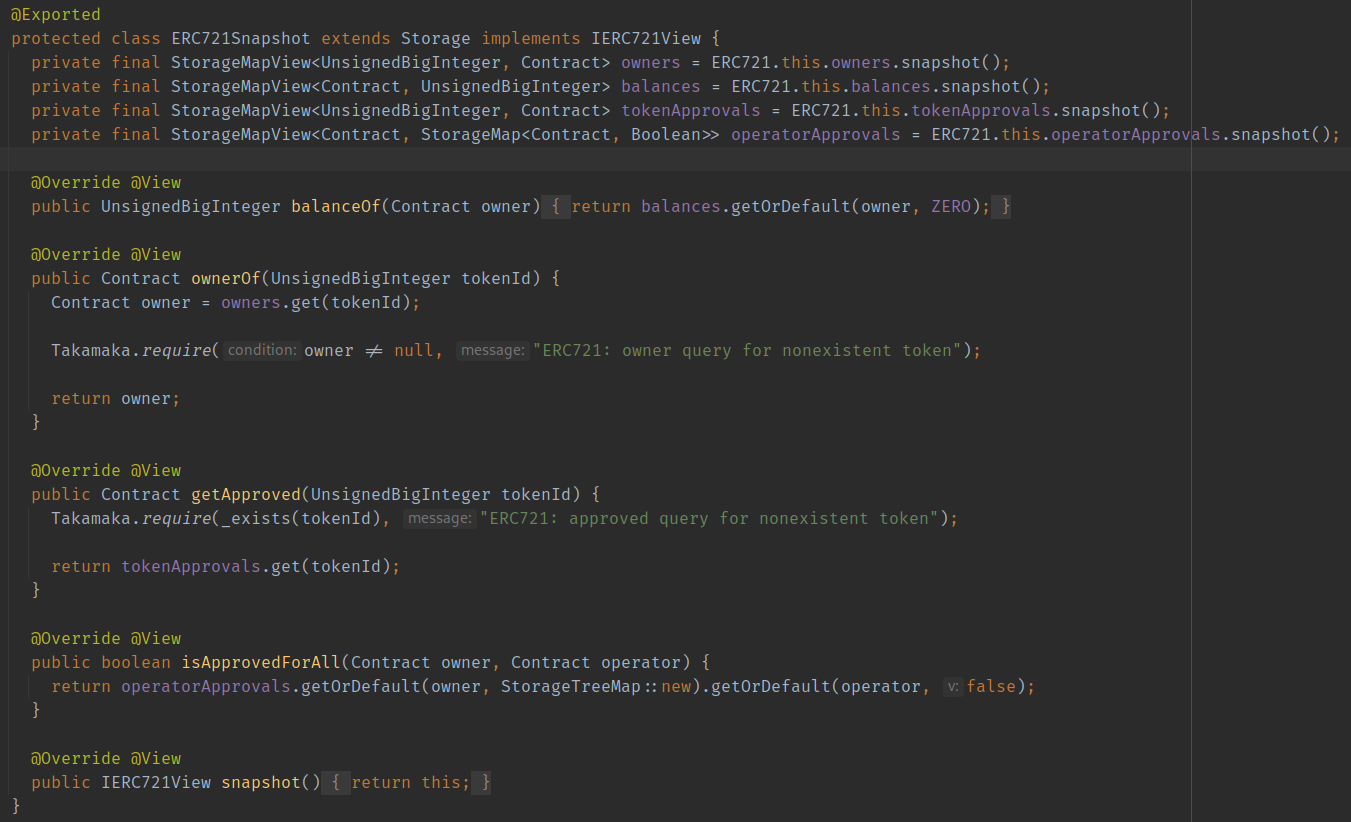
\includegraphics[width=0.8\textwidth]{capitolo3/erc721-hotmoka/erc721-hotmoka-snapshot.png}
  \caption{Implementazione del sistema dello \textit{Snapshot} di un oggetto di tipo ERC721}
  \label{fig:erc721-snapshot}
\end{figure}


\subsection{Verifica}
Per quanto concerne la verifica dello standard ERC721 per Hotmoka, in seguito ad una discussione con il mio \textit{tutor} aziendale, Fabio Pallaro, è stato deciso che non c'è il bisogno di verificare attraverso la scrittura di \textit{test} automatici anche questa parte del progetto. La seguente scelta è stata presa perché, inizialmente non era prevista la scrittura dello standard ERC721 per Hotmoka e, in più, non c'era abbastanza tempo per poterli implementare.
